\documentclass[11pt]{amsbook}

\usepackage{../HBSuerDemir}	% ------------------------
\usepackage{graphicx,wrapfig,lipsum}


\begin{document}

% ++++++++++++++++++++++++++++++++++++++
\hPage{b2p2/328}
% ++++++++++++++++++++++++++++++++++++++

The largest (smallest) element M(m) in $R_{f}$, if any, is the \textit{global} or \textit{absolute maximum (minimum)} of f over $D_{f}$.
\\

If $f\left ( P_{0} \right ) \in R_{f} $ is the largest (smallest) in a neighborhood $N(P_{0})$ of a point $P_{0} \in D_{f} $, then $f\left ( P_{0} \right )$ is \textit{local} or \textit{relative maximum(minimum)} of f at $P_{0}$, and $P_{0}$is said to be an \textit{extremum point} of f. Since no conditions are imposed on the independent variables (variables varying freely) the extrema will be called a \textit{free extrema}.
\\

For the global maximum (minimum) of f at a point $P_{0}$, one has 
\\

$f\left ( P_{0} \right ) \geq f\left ( P \right )$ $(  f\left ( P_{0} \right ) \leq  f\left ( P \right ))$ for all $P \in D_{f}$, while for a maximum (minimum) of at $P_{0}$,
\begin{center}
$f\left ( P_{0} \right ) \geq f\left ( P \right )$ $(  f\left ( P_{0} \right ) \leq  f\left ( P \right ))$ for all $P \in N(P_{0})$.
\end{center}

DETERMINATION OF LOCAL EXTREMA (for a function of two variables)

Let $z= f(x, y)$ be a function of two variables defined on D. If its first partial derivatives exist and both zero at $P_{0}(a, b) \in D $, 
\begin{wrapfigure}{r}{3cm}
	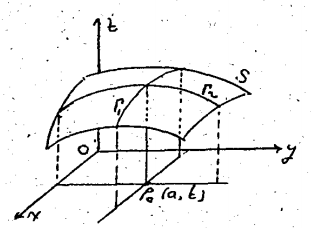
\includegraphics[width=4cm]{images/b2p2-328-fig01.png}
\end{wrapfigure} 
then by the geometric interpretations of $f_{x}(P_{0})$, $f_{y}(P_{0})$, the point $P_{0} $ is a critical point of both of the curves 


\begin{align*}
r_{1: } &  y  = b,   z = f(x, y)      \\
r_{2: } &  x  = a,   z = f(x, y)
\end{align*}


If f has a local extrema at $P_{0}$, then $f_{x}$, $f_{y}$ vanish both at $P_{0}$ as stated in the following theorem.
\\

A point $P_{0}$ at which partial derivatives $f_{x}$, $f_{y}$ vanish simultaneously is called a \textit{critical point} of $f(x, y)$.


% =======================================================
\end{document}  
